\chapter{OLS 回归的解释}
\label{ch:week2}
\section{简单普通最小二乘回归}
\sourcepage{2}{1}{2/1}
\label{sec:simple-interpretation}
\subsection{模型与其他条件不变的解释}
简单回归模型为
\begin{equation}\label{eq:simple-model}
 y_i=\beta_0+\beta_1x_i+u_i.
\end{equation}
对另一观测，有 $y_{i'}=\beta_0+\beta_1x_{i'}+u_{i'}$。不同观测对应不同的 $u$；因此不能只因 $x$ 不同就把 $y$ 的全部变化归于 $x$。
将两个方程相减，得到
\[\hm{\Delta y=\beta_1\Delta x+\Delta u}.\]
若 $u$ 保持不变，则 $y$ 的变化等于 $x$ 的变化乘以 $\beta_1$：
\[\Delta u=0\quad\Longrightarrow\quad
\hy{$\Delta y=\beta_1\Delta x$},\qquad
\beta_1=\frac{\Delta y}{\Delta x}\quad(\Delta x\ne0).\]
\textbf{解释。}\hy{其他条件不变时}，$x$ 增加一个单位，与 $y$ 增加 $\beta_1$ 个单位相对应。在这一线性模型中，保持 $u$ 不变时，$\beta_1$ 是 \hy{$x$ 对 $y$ 的边际效应}。如果系数为负，“增加”应理解为相应的减少。

\subsection{关于误差的假设}
\begin{enumerate}
\item \hy{$\E[u]=0$}：误差的均值为零。若截距不受限制，可通过归一化满足这一条件。若 $\E[u]=\alpha$，令 $\varepsilon=u-\alpha$，则 $\E[\varepsilon]=0$，并且
\[y=\beta_0+\beta_1x+u=(\beta_0+\alpha)+\beta_1x+\varepsilon.\]
截距吸收了误差中非零的均值；这一操作本身并不能建立外生性。\corr{mean-normalisation}
\item \hy{零条件均值（ZCM）}假设：
\begin{equation}\label{eq:zcm-simple}
\hm{\E[u\mid x]=0}.
\end{equation}
$u$ 的条件期望不随 $x$ 的取值而变。结合前面的均值归一化，有 $\E[u\mid x]=\E[u]=0$。原稿亦称其为\hy{外生性假设}。
\end{enumerate}
\begin{example}[教育与工资]
\[\wage=\beta_0+\beta_1\educ+u.\]
未观测因素包括智力、家庭背景、经验和培训等。在 ZCM 下，无论教育年限为 12 年还是 16 年，未观测因素 $u$ 的\emph{条件平均值}都相同；这并不意味着每个人的能力和背景完全相同。
\blue{现实中很难控制所有未观测因素。}能力、背景可能与教育相关，因此这一假设并非天然合理。\red{随机分配可以帮助建立外生性}，但仍须结合实际研究设计核查。
\end{example}
% The rest of this chapter is appended after the GPA example below.

\subsection{总体回归函数与拟合回归线}
\sourcepage{2}{2}{2/2}
在式 \eqref{eq:zcm-simple} 成立时，\hy{总体回归函数（PRF）}为
\begin{align}
\E[y\mid x]
&=\E[\beta_0+\beta_1x+u\mid x] \notag\\
&=\E[\beta_0+\beta_1x\mid x]+\E[u\mid x] \notag\\
&=\hm{\beta_0+\beta_1x}.\label{eq:prf}
\end{align}
给定 $x$ 后，$\beta_0+\beta_1x$ 为常数。其中 $\beta_0$ 是截距，$\beta_1$ 是总体回归函数的斜率。在这一简单的水平值—水平值模型中，总体回归函数对 $x$ 呈线性。
\begin{figure}[htbp]
\centering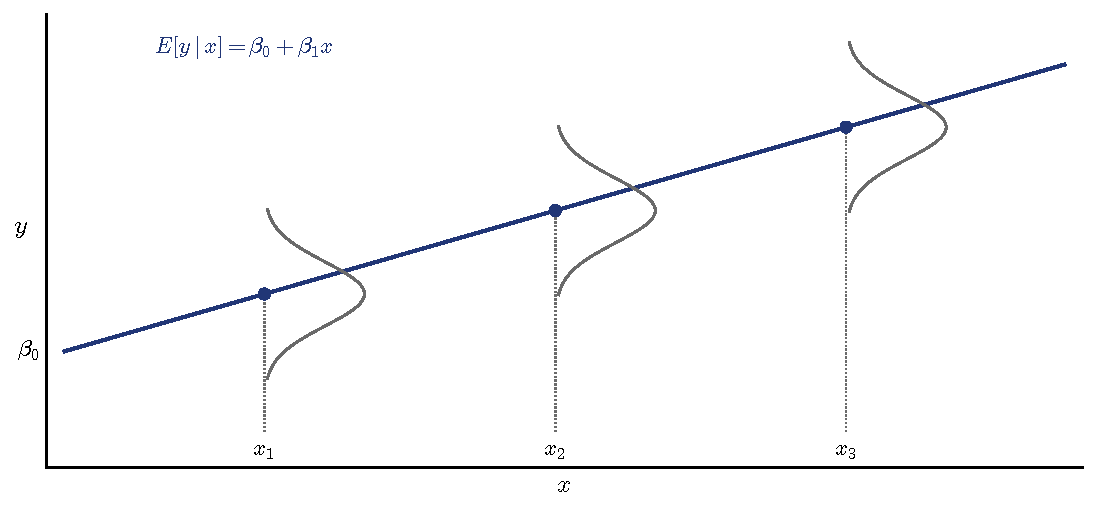
\includegraphics[width=.82\linewidth]{conditional_means.pdf}
\caption{不同 $x$ 取值下的总体条件均值。侧面的曲线表示条件分布；本图为教学示意，不是实际观测数据。}
\label{fig:conditional-means}
\end{figure}
\paragraph{普通最小二乘法（OLS）。}
\textbf{拟合回归线}，亦称样本回归线，为
\begin{equation}\label{eq:fitted-simple}
\hat y_i=\hat\beta_0+\hat\beta_1x_i,
\qquad \hat\beta_0=\bar y-\hat\beta_1\bar x.
\end{equation}
若样本中的 $x$ 存在变异，则
\begin{equation}\label{eq:simple-slope}
\hm{\hat\beta_1=
\frac{\sum_i(x_i-\bar x)(y_i-\bar y)}{\sum_i(x_i-\bar x)^2}
=\frac{\Cov_n(x,y)}{\Var_n(x)}
=r_{xy}\frac{s_y}{s_x}}.
\end{equation}
其中 $r_{xy}=\Cov_n(x,y)/(s_xs_y)$。分子与分母采用一致的协方差归一化约定。\corr{slope-correlation}

\textbf{斜率。}其他条件不变时，$x$ 增加一个单位，\hy{与 $y$ 的预测值增加 $\hat\beta_1$ 个单位相关联}。
\blue{原稿例式：$y=\beta_0+\beta_1x+\beta_2z+\beta_3w+u$；若 $z,w$ 遗漏，简单回归系数可能把它们的影响一并算入。}

\red{相关不等于因果。}缺少合理的数据生成过程和识别假设时，应使用“相关联”或“相关”等措辞，而不应使用“导致”“使得”等因果表述。若模型具有可辩护的结构性、外生性及因果识别条件，才可进一步解释为因果效应。\corr{causality}

\textbf{截距。}$x=0$ 时，$y$ 的拟合值为 $\hat\beta_0$；在式 \eqref{eq:prf} 成立时，$x=0$ 处的总体条件均值为 $\beta_0$。若零不在观测范围或可行范围内，这一解释可能只是外推。

拟合线取决于样本；总体回归线则固定但未知。原稿中薪酬与净资产收益率的例式保留为
\[\widehat{\mathrm{salary}}=963.191+18.501\,\mathrm{roe}.\]
\begin{figure}[htbp]
\centering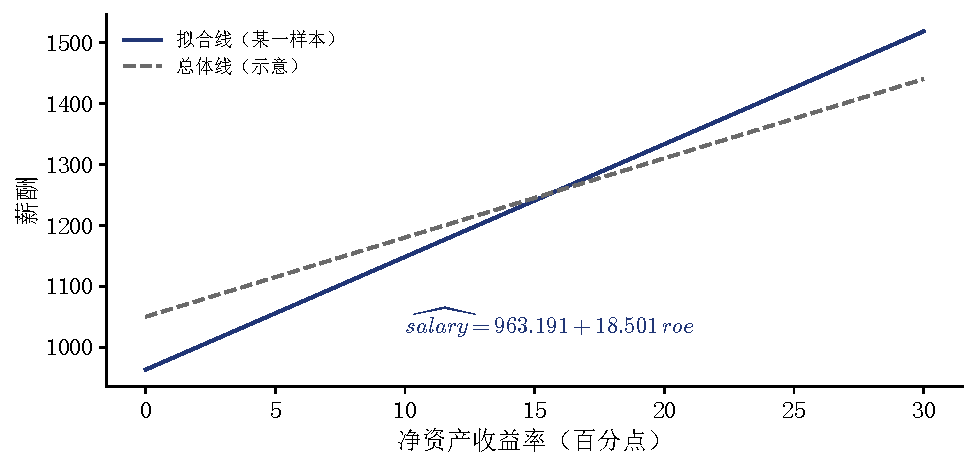
\includegraphics[width=.8\linewidth]{fitted_population.pdf}
\caption{拟合回归线与总体回归线的比较，沿用原稿中薪酬与净资产收益率的示意。总体线仅作示意，并非另行估计的基准。}
\label{fig:fitted-population}
\end{figure}

\subsection{例题：单位与百分点}
\sourcepage{2}{3}{2/3}
\begin{example}[小时工资：注意单位]\label{ex:wage-units}
原题将小时工资的单位规定为\hy{千美元}，教育年限的单位为年：
\[\wage=\beta_0+\beta_1\educ+u,\qquad
\widehat{\wage}=-0.9+0.54\educ.\]
安森每小时挣 6 美元，受教育年限为 12 年。若保持未观测因素不变，当其受教育年限变为 16 年时，模型给出的情景工资是多少？
\begin{align*}
\widehat{\wage}_{12}&=-0.9+0.54(12)=5.58\quad\text{（千美元/小时）},\\
\hat u_{\text{安森}}&=0.006-5.58=-5.574,\\
\Delta\widehat{\wage}&=0.54(16-12)=2.16\quad\text{（千美元/小时）},\\
\widehat{\wage}_{16}&=-0.9+0.54(16)=7.74.
\end{align*}
在本题的模型情景中，若将拟合残差保持不变，则
\[\wage_{16}^{\text{情景}}=7.74-5.574=2.166,
\qquad\text{即每小时 }2{,}166\text{ 美元}.\]
等价地，
\[\hp{情景工资 = 原实际工资 + 模型给出的变化量},\]
\[\$6+(\$0.54\times10^3\times4)=\$2{,}166.\]
\added{数值异常大，是因为原稿明确采用了\emph{千美元}的单位；本笔记没有擅自将单位改成美元。固定某个人的误差或拟合残差，只是一项假设情景，不代表已经识别出的个体反事实，也不能保证其未来的实际工资。}\corr{wage-counterfactual}
\end{example}

\begin{exercise}[竞选支出]\label{ex:election}
\[\widehat{\mathrm{voteA}}=26.81+0.464\,\mathrm{shareA}.\]
其中，$\mathrm{voteA}$ 表示候选人 A 的得票百分比；$\mathrm{shareA}$ 表示 A 的竞选支出占两位候选人总支出的百分比。支出占比每增加一个\hy{百分点}，与预测得票率增加 0.464 个百分点相关联。
\begin{enumerate}
\item 若支出占比为 $40\%$，应代入 $40$，而不是 $0.40$：
\[\widehat{\mathrm{voteA}}=26.81+0.464(40)=\hm{45.37\%}.\]
若 A 完全不支出，拟合值为 $26.81$；若 A 承担全部支出，则为 $26.81+0.464(100)=73.21$。这些是拟合线给出的预测，不能保证选举结果。
\item 若候选人 B 支出 20 亿美元，A 至少需要达到怎样的支出门槛，才能使\emph{预测}得票率超过 $50\%$？
\begin{align*}
26.81+0.464\,\mathrm{shareA}&>50,\\
\mathrm{shareA}&>\frac{23.19}{0.464}=49.978448\ldots.
\end{align*}
\added{令 $A$ 表示以十亿美元为单位的支出。由于 $\mathrm{shareA}=100A/(A+2)$，有
\[A>\frac{2(49.978448\ldots)}{100-49.978448\ldots}
=1.9982766\ldots\ \text{十亿美元}.\]
严格不等式给出的是支出门槛；在连续支出范围内，该门槛并不是能够取到的最小值。此回归不能保证实际获胜。}\corr{election}
\end{enumerate}
\end{exercise}

\section{多元 OLS 的解释}
\sourcepage{2}{4}{2/4}
\label{sec:multiple-interpretation}
总体模型与拟合方程分别为
\begin{align}
y&=\beta_0+\beta_1x_1+\cdots+\beta_kx_k+u,\label{eq:multiple-model}\\
\hat y&=\hat\beta_0+\hat\beta_1x_1+\cdots+\hat\beta_kx_k.\label{eq:multiple-fitted}
\end{align}
对一个给定的拟合方程，有
\[\hm{\Delta\hat y=\hat\beta_1\Delta x_1+\cdots+\hat\beta_k\Delta x_k}.\]
保持其余 $x_j$ 全部不变，得到
\[\Delta\hat y=\hat\beta_\ell\Delta x_\ell,
\qquad\frac{\Delta\hat y}{\Delta x_\ell}=\hat\beta_\ell.
\]
\textbf{偏效应。}在总体模型中，保持其余回归变量\emph{以及} $u$ 不变时，$\beta_\ell=\Delta y/\Delta x_\ell$；在 ZCM 下，它也是 $\E[y\mid x_1,\ldots,x_k]$ 对该变量的偏斜率。\corr{notation}
\[\hy{$\E[u\mid x_1,\ldots,x_k]=0$}.\]
将其他解释变量纳入回归，就可以在拟合比较中保持其观测值不变。\blue{不需要 $x_\ell$ 与其他 $x_j$ 互不相关；只需避免完全共线性，才能区分各自系数。}

\begin{example}[大学平均绩点]\label{ex:gpa}
\[\widehat{\colGPA}=1.29+0.453\hsGPA+0.0094\ACT.\]
原稿给定的范围为：大学平均绩点 $\colGPA$ 为 $0$--$4$，高中平均绩点 $\hsGPA$ 为 $1$--$4$，ACT 考试分数为 $0$--$36$。
\begin{description}
\item[高中绩点。]保持 ACT 分数及其他因素不变，高中平均绩点每提高 1 分，与大学平均绩点的预测值提高 0.453 分相关联。
\item[ACT 分数。]保持高中平均绩点及其他因素不变，ACT 分数每提高 1 分，与大学平均绩点的预测值提高 0.0094 分相关联。
\item[截距。]高中绩点与 ACT 分数都为零时，大学平均绩点的拟合值为 $1.29$。\red{高中绩点为零超出了题定范围}，因此这只是外推，并非对某个已观测群体的预测。
\end{description}
\begin{enumerate}
\item 若 ACT 分数固定，高中绩点从 $3.5$ 升至 $3.6$，则
\[\Delta\widehat{\colGPA}=(3.6-3.5)(0.453)=0.0453.\]
\item 安森的高中绩点为 $3.5$、ACT 为 $30$；贝蒂的高中绩点为 $3.0$、ACT 为 $36$：
\begin{align*}
\widehat{\colGPA}_{A}&=1.29+0.453(3.5)+0.0094(30)=3.1575,\\
\widehat{\colGPA}_{B}&=1.29+0.453(3.0)+0.0094(36)=2.9874.
\end{align*}
\item 若安森的实际大学绩点为 $3.3$，能否推断贝蒂的实际绩点？不能。\blue{每个人的 $u$ 不同，不能由一个人的实际值推出另一个人的实际值。}安森在本样本中的残差为 $3.3-3.1575=0.1425$；贝蒂的残差未知。
\end{enumerate}
\end{example}


\section{控制变量与 FWL 定理}
\sourcepage{2}{5}{2/5}
\label{sec:fwl-week2}
\subsection{为什么引入控制变量？}
假设我们关心教育年限 $x_1$ 对工资 $y$ 的影响，而能力 $x_2$ 也会影响工资：
\[y=\beta_0+\beta_1x_1+\beta_2x_2+u.\]
若遗漏能力，短方程 $y=\tilde\beta_0+\tilde\beta_1x_1+v$ 可能将能力的影响归到教育上。当能力既影响工资又与教育相关时，这就涉及\hp{遗漏变量偏误}。

“控制”可以从两个角度理解：
\begin{enumerate}
\item \hy{保持不变}：保持 $x_2$ 固定，比较 $x_1$ 的变化。
\item \hy{剔除线性影响}：先移除能够由 $x_2$ 线性解释的部分，再解读 $x_1$ 的系数。
\end{enumerate}
\blue{二者描述的是同一个多元回归系数；FWL 将“排除其他变量的线性影响”写成可计算的步骤。}

\subsection{将回归变量残差化}
在样本中，先将 $x_1$ 对常数项与 $x_2$ 回归：
\begin{equation}\label{eq:fwl-x}
x_{1i}=\hat\delta_0+\hat\delta_1x_{2i}+\hat r_{1i}.
\end{equation}
残差 $\hat r_{1i}$ 是 $x_{1i}$ 中\hy{不能由 $x_2$ 线性解释的部分}，并满足
\[\sum_i\hat r_{1i}=0,\qquad\sum_i x_{2i}\hat r_{1i}=0.\]
再将 $y_i$ 对常数项与 $\hat r_{1i}$ 回归，其斜率恰好等于原多元 OLS 中 $x_1$ 的系数：
\begin{equation}\label{eq:fwl-one-sided}
\hm{\hat\beta_1=
\frac{\Cov_n(\hat r_1,y)}{\Var_n(\hat r_1)}
=\frac{\sum_i\hat r_{1i}y_i}{\sum_i\hat r_{1i}^2}}.
\end{equation}
因此，$\hat\beta_1$ 描述的是：剔除 $x_1$ 与 $x_2$ 的线性关系后，$x_1$ 的剩余变化与 $y$ 之间的拟合关系。\blue{将 $x_1$ 对控制变量回归，留下不被它们线性解释的部分。}

\added{标准的双侧 FWL 回归还需将 $y$ 对 $(1,x_2)$ 回归，得到 $\hat r_{yi}$，再将 $\hat r_y$ 对 $\hat r_1$ 作无截距回归。所得斜率\emph{与残差}均和完整模型相同。原稿中的单侧回归给出相同斜率，但通常不会给出相同的回归残差。}\corr{fwl-residual}

\subsection{一般情形}
对 $y=\beta_0+\beta_1x_1+\cdots+\beta_kx_k+u$，将 $x_1$ 对 $(1,x_2,\ldots,x_k)$ 回归：
\[x_{1i}=\hat\delta_0+\hat\delta_2x_{2i}+\cdots+\hat\delta_kx_{ki}+\hat r_{1i}.\]
将 $y_i$ 对 $\hat r_{1i}$ 与常数项回归；也可将经过相应残差化的 $y_i$ 对 $\hat r_{1i}$ 作无截距回归。只要残差变异为正，式 \eqref{eq:fwl-one-sided} 仍成立。更多细节及原稿重复的推导保留在\hyperref[sec:fwl-week3]{第 3 周}和\hyperref[sec:fwl-week4]{第 4 周}。

\section{简单回归与多元回归的斜率比较}
\sourcepage{2}{6}{2/6}
\label{sec:short-long-week2}
增加一个控制变量时，它必须与原回归变量不相关吗？\red{不用！}控制变量与原变量相关，恰恰是简单与多元回归斜率经常不同的原因。但控制变量应适合所研究的因果或预测问题；加入它并不自动消除偏误。

考虑以下总体方程：
\begin{align*}
y&=\beta_0+\beta_1x_1+\beta_2x_2+u,\\
x_2&=\delta_0+\delta_1x_1+\varepsilon.
\end{align*}
第二个方程是总体线性投影，满足 $\E[\varepsilon]=\E[x_1\varepsilon]=0$。若 $\E[u\mid x_1,x_2]=0$，代入可得
\begin{align*}
y&=\beta_0+\beta_1x_1+\beta_2(\delta_0+\delta_1x_1+\varepsilon)+u\\
 &=\underbrace{(\beta_0+\beta_2\delta_0)}_{\tilde\beta_0}
  +\underbrace{(\beta_1+\beta_2\delta_1)}_{\tilde\beta_1}x_1
  +\underbrace{(u+\beta_2\varepsilon)}_{v}.
\end{align*}
因此，短模型的总体投影斜率为
\begin{equation}\label{eq:population-ovb}
\hm{\tilde\beta_1=\beta_1+\beta_2\delta_1}.
\end{equation}
这是\emph{总体投影系数}之间的关系，不能写成估计量与固定总体参数之间的相等关系。\corr{ovb-levels}

\paragraph{两个斜率何时相同？}
在含两个回归变量的情形中，$\tilde\beta_1=\beta_1$ 当且仅当 $\beta_2\delta_1=0$：
\begin{enumerate}
\item $\beta_2=0$：$x_2$ 对 $y$ 的偏效应为零；即使 $x_1$ 与 $x_2$ 相关，两个总体斜率仍相同。
\item $\delta_1=0$：$x_1$ 与 $x_2$ 在总体中不相关。
\end{enumerate}
\added{对于具体样本中的 OLS 系数，精确的样本恒等式为
\[\hat{\tilde\beta}_1=\hat\beta_1+\hat\beta_2\hat\delta_1.\]
因此，若 $\hat\beta_2=0$，或\emph{样本}辅助回归斜率 $\hat\delta_1=0$，两个样本斜率相同。总体系数为零，并不强制其样本估计值恰好为零。}

\begin{example}[平均绩点：控制变量改变系数解释]\label{ex:gpa-short-long}
比较以下经过舍入的拟合方程：
\begin{align*}
\widehat{\colGPA}&=1.29+0.453\hsGPA+0.0094\ACT,\\
\widehat{\colGPA}&\simeq2.40+0.0271\ACT
                       &&\text{（仅含 ACT）},\\
\widehat{\hsGPA}&\simeq2.46+0.039\ACT,\\
\widehat{\colGPA}&\simeq1.41+0.482\hsGPA
                       &&\text{（仅含高中绩点）}.
\end{align*}
以 ACT 为例，以下舍入数值的运算体现了总体或样本方程相互代入的直觉：
\[1.29+0.453(2.46)=2.40438,\qquad
0.0094+0.453(0.039)=0.027067\simeq0.0271.\]
仅含高中绩点的斜率与其多元回归斜率较接近，部分原因是 ACT 的偏回归系数较小。\blue{小的遗漏系数只有与辅助回归系数的大小一起看，才说明偏差是否小。}以上方程均为原稿中经过舍入的例子，并非重新估计的实证结果。
\end{example}

\section{计量单位与函数形式}
\sourcepage{2}{7}{2/7}
\label{sec:units}
\subsection{改变因变量的计量单位}
从 $y=\beta_0+\beta_1x+u$ 出发。若 $y'=cy$ 且 $c\ne0$，则
\[y'=c\beta_0+c\beta_1x+cu.\]
因此，
\[\hy{$\beta'_0=c\beta_0$},\qquad
\hy{$\beta'_1=c\beta_1$},\qquad u'=cu,\qquad\Delta y'=c\Delta y.\]
例如，从美元换算为千美元时，$c=1/1000$。
样本 OLS 的推导为
\begin{align*}
\hat\beta'_1
 &=\frac{\Cov_n(x,y')}{\Var_n(x)}
 =\frac{\Cov_n(x,cy)}{\Var_n(x)}
 =c\hat\beta_1,\\
\hat\beta'_0
 &=\bar y'-\hat\beta'_1\bar x
 =c\bar y-c\hat\beta_1\bar x=c\hat\beta_0.
\end{align*}
在 ZCM 下，$x=0$ 处的截距解释变为
\[\E[y'\mid x=0]=c\beta_0=\beta'_0.\]
\red{这里必须写条件均值；通常不能写成 $\beta_0=\E[y]$。}一般地，当 $\E[u]=0$ 时，$\E[y]=\beta_0+\beta_1\E[x]$。\corr{unit-intercept}

\subsection{改变回归变量的计量单位}
若 $x'=cx$ 且 $c\ne0$，则
\[y=\beta_0+\frac{\beta_1}{c}x'+u,\qquad
\hy{$\beta'_0=\beta_0$},\quad\hy{$\beta'_1=\beta_1/c$}.\]
$x'=0$ 时也有 $x=0$，因此截距不变。对拟合系数，有
\begin{align*}
\hat\beta'_1
 &=\frac{\Cov_n(x',y)}{\Var_n(x')}
 =\frac{c\Cov_n(x,y)}{c^2\Var_n(x)}
 =\frac{\hat\beta_1}{c},\\
\hat\beta'_0&=\bar y-\frac{\hat\beta_1}{c}(c\bar x)=\hat\beta_0.
\end{align*}
相应的拟合均值恒等式为 $\bar y=\hat\beta'_0+\hat\beta'_1\bar x'$。

\section{水平值与对数模型}
\sourcepage{2}{8}{末页}
\label{sec:logs}
\blue{水平值对应单位变化；对数对应相对或百分比变化。}以下对数均为自然对数，要求真数为正。比较时始终保持误差与其他回归变量不变。普通有限百分比变化记为 $\%\Delta x=100\Delta x/x_0$ 和 $\%\Delta y=100\Delta y/y_0$。

\subsection{水平值—水平值模型}
\[y=\beta_0+\beta_1x+u,\qquad
\hm{\Delta y=\beta_1\Delta x}.\]
$x$ 每增加一个单位，对应 $y$ 增加 $\beta_1$ 个单位。

\subsection{水平值—对数模型}
\[y=\beta_0+\beta_1\ln x+u,\qquad
\frac{dy}{d\ln x}=\beta_1,\qquad
dy=\beta_1\frac{dx}{x}.\]
对于较小的变化，
\[\hm{\Delta y\approx\frac{\beta_1}{100}\,\%\Delta x}.\]
$x$ 增加百分之一，与 $y$ 大约增加 $\beta_1/100$ 个单位相对应。
\added{对于有限变化，模型的精确关系为 $\Delta y=\beta_1\ln(x_1/x_0)$。当 $x$ 增加 $1\%$ 时，变化量为 $\beta_1\ln(1.01)$，并不恰好等于 $\beta_1/100$。}\corr{logs}

\subsection{对数—水平值模型}
\[\ln y=\beta_0+\beta_1x+u,\qquad
\frac{d\ln y}{dx}=\beta_1=\frac{1}{y}\frac{dy}{dx}.\]
因此，$\beta_1$ 是以小数表示的半弹性，且
\[\hm{\%\Delta y\approx100\beta_1\Delta x}.\]
$x$ 每增加一个单位，对应 $y$ 的变化率约为 $100\beta_1\%$。
\added{对于有限的 $\Delta x$，在保持误差不变时，精确关系为
\[\%\Delta y=100\bigl(e^{\beta_1\Delta x}-1\bigr).\]
将 $\E[\ln y\mid x]$ 取指数，一般不等于 $\E[y\mid x]$；若要解释水平值的条件均值，还需要进行反变换调整。}\corr{logs}

\subsection{对数—对数模型}
\[\ln y=\beta_0+\beta_1\ln x+u,\qquad
\hm{\beta_1=\frac{d\ln y}{d\ln x}
=\frac{dy/y}{dx/x}}.\]
$\beta_1$ 是弹性。对于较小的变化，
\[\%\Delta y\approx\beta_1\,\%\Delta x.\]
$x$ 增加百分之一，对应 $y$ 大约变化 $\beta_1\%$。
\added{对于普通有限百分比变化 $p=\%\Delta x$，
\[\%\Delta y=100\left[\left(1+\frac p{100}\right)^{\beta_1}-1\right].\]
微分形式的弹性关系是精确的；将微分替换为任意有限变化，则属于近似。}\corr{logs}

\subsection*{本章小结}
\addcontentsline{toc}{subsection}{本章小结}
\begin{itemize}
\item 拟合斜率描述预测上的关联；因果解释还需要恰当的模型与研究设计。
\item 多元 OLS 在比较中保持已纳入的控制变量不变；FWL 通过残差化提取同一个斜率。
\item 单位变化会相应缩放系数。解释对数模型时，须明确区分精确关系与百分比近似。
\end{itemize}
